%\vspace{-2ex}
\section{Translating memory locations to symbols}
%\vspace{-2ex}
\label{sec:symprom}
%In x86, the shortage of architectural registers yields an especially large number of memory operations. Promotion of these memory locations to symbols is imperative for effectiveness of traditional compiler analysis in a rewriter. 
Sec~\ref{sec:deconstructFrame} presented methods for deconstructing the physical stack frame into individual abstract frames, one per procedure. Even though this representation allows unrestricted modification of the stack frame, accesses to local variables appear as explicit memory references to locations within this array, which are not amenable to standard data-flow analysis. In this section, we propose our methods for translating these memory operations to symbol operations in the IR.

%\subsection{Limitations of variable identification}
%Commercial disassembly tools like IDAPro~\cite{ida-pro} identify statically determinable stack-frame offsets in the program as local variables. More advanced tools like Divine~\cite{reps06} identify variables from the stack offsets present in the value set of the data objects.
                                                                        
\begin{figure}[t]
{
\vspace{-0.2in}
\centering
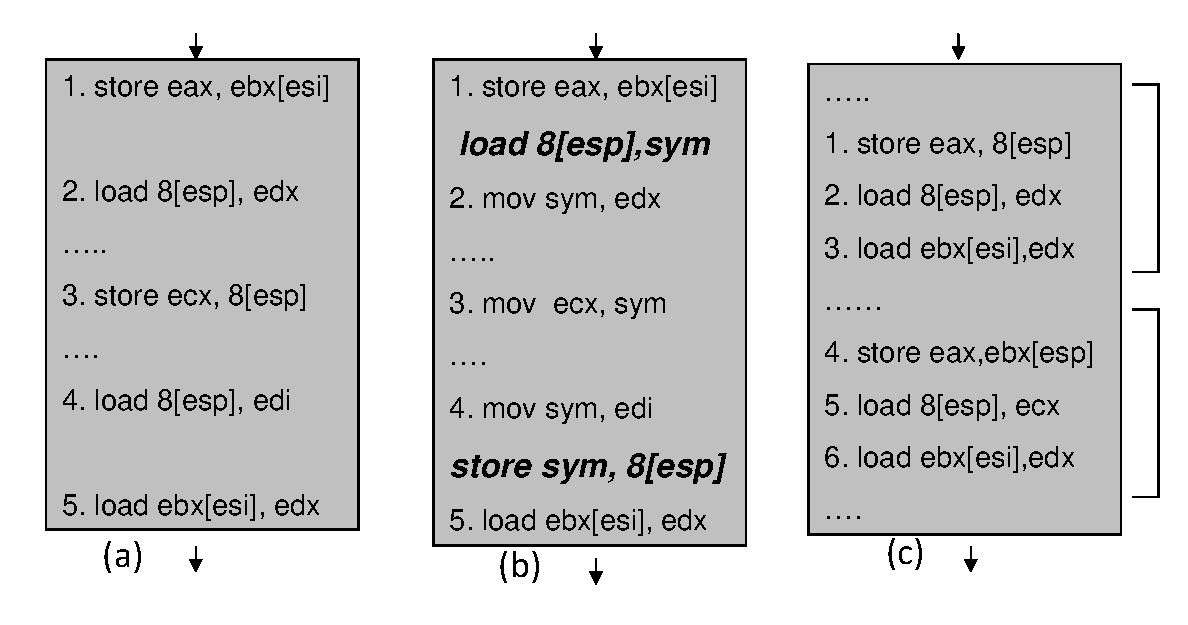
\includegraphics[width=0.7\linewidth]{figures/EPS/pathcfg.eps}
\vspace{-2ex}
\caption{\textit{Symbol promotion. Second operand in the instruction is the destination of the instruction. }}
\label{fig:PromExample}
}
\vspace{-3ex}
\end{figure}






\subsection{Motivation for partitions}

%We need to ensure that the symbol contains the latest data-flow-consistent value for the memory location after any aliasing definition and the memory location contains the latest value consistent with data-flow before we execute an aliasing use. 
As presented in Sec~\ref{sec:contributions}, maintaining the data-flow consistency of the underlying memory locations across the whole program is imperative while promoting memory accesses to symbolic accesses. Fig~\ref{fig:PromExample}(a) shows a small example with three direct accesses to location \emph{(esp+8)} at Lines 2,3,4; the remaining two are unbounded indirect accesses. The simplest method for maintaining the data-flow consistency across the program is to load the data from the memory location into the symbol just after each aliasing definition, store the symbol back to the memory location just before each aliasing use and promote each candidate stack access to a symbolic access, as shown in Fig~\ref{fig:PromExample}(b). The load inserted just after the aliasing definition is referred to as a \emph{Promoting Load} and store just before the aliasing use is referred to as a \emph{Promoting Store} (shown as bold in Fig~\ref{fig:PromExample}(b)). Although this method ensures correct data flow propagation, it results in a large number of promoting loads and stores which might overshadow the benefit of symbol promotion.
%The insertion of promoting loads and stores ensure that the data-flow is maintained correctly and the intermediate direct memory accesses can safely be replaced by symbol accesses. 


\begin{figure}[t]
{
\vspace{-0.2in}
\centering
{
\begin{scriptsize}
\begin{tabular}{|c|c|c|} %|r|r|r|}
%xxxxx\=xxxxxxxxxxxxx\=xxxxxx\=xxxxxxxxxxx\=xxxxxx\=  \kill\\
\hline
\textbf{Statement s}&\textbf{gen[s]}&\textbf{kill[s]}\\ \hline
d:store x,mem[reg]&if([sp+addr]$\in$VS(mem+reg))&if([sp+addr]$\in$VS(mem+reg))\\	
					     &				d 	&				defs(addr) - {d}\\ 
					     &	else \{ \} 	&				else \{ \}\\ \hline
d: store y,addr[sp]&					d	&			defs(addr) - {d}\\ \hline
d: z = load mem[reg]& \{\}&  \{\}\\ \hline
d: z = load addr[sp]&\{\}&	\{\} \\ \hline
\end{tabular}
\begin{tabbing}
Memory location $loc: [sp + addr]$ \\
$mem$: Non-constant access\\
$addr$: Constant\\
$defs(addr)$: Set of instructions defining the memory location [sp+addr]\\
$in[n]$: Set of definitions that reach the begining of node n \\
$out[n]$: Set of definitions that reach  the end of node n \\
$pred[n]$: Predecessor nodes of node n\\
$in[n] = \cup_{i | i \in pred[n]}\{ (out[p])\}$ \\
$out[n] = gen[n] \cup (in[n] - kill[n])$
%\line(1,0){220}
\end{tabbing}
\caption {\textit{The reaching definition description. Definitions are propagated across the control flow of program }}
\label{fig:reachingdef}
\end{scriptsize}
\vspace{-2ex}
}
}
\end{figure}

%Unprofitable case - extra load/stores
Fig~\ref{fig:PromExample}(c) illustrates this unprofitable case. In this example, suppose VS of \emph{ebx} is TOP. Consequently, the instructions at Line 3, 4 and 6 are aliasing indirect accesses to the stack location \emph{(sp+8)}. In order to promote the direct memory accesses at instructions 1, 2 and 5, we need to insert Promoting Stores just before instruction 3 and instruction 6 and a Promoting Load just after instruction 4. Hence, promoting three direct memory operations entails the insertion of three extra memory operations, nullifying the benefit. 

%Need for partition
We propose a novel partition-based symbol promotion algorithm where we divide the program into a set of non-overlapping promotional lifetimes for each memory location. It serves as a fine-grain framework where the symbol promotion decision can be made independently for each lifetime (a partition) instead of the entire program at once. Not doing symbol promotion in a partition does not affect the correctness of the data-flow in the program. The symbol promotion can be selectively performed in only those partitions where it is provably beneficial. Fig~\ref{fig:PromExample}(c) shows an intuitive division of the current example into two safe partitions.

%Partitions are computed based on a reaching definition framework defined on the memory accesses. Next, we present our reaching definition framework for computing the partitions.

\subsection{Reaching definition framework}

We define a new reaching definition analysis on \emph{memory locations} for computing the partitions. This is different from the standard reaching definitions on \emph{symbols} well-known in compiler theory. For each memory location \emph{loc}, this analysis computes the set of instructions defining the memory location \emph{loc} that reach each program point. The set of definitions includes stores to the memory location \emph{loc} using direct addressing mode as well as possibly aliasing stores.

%ValueSet TOP represents that the memory access instruction aliases with any memory location.
Fig~\ref{fig:reachingdef} formulates the reaching definition in terms of VS of the memory accesses. These reaching definitions are propagated across the control flow of the program, similar to the standard compiler dataflow propagation, allowing the partitions to be formed across basic blocks. The interprocedural version of VSA implicitly takes into consideration a local pointer passed to a procedure through an argument.
%For a memory access instruction \emph{m}, we define \emph{$dest_{m}$} as its underlying destination. $ValueSet(dest_{m})$, as determined by VSA, represents the possible memory locations which can be accessed by the memory access instruction \emph{m}.  

\subsection{Symbol promotion algorithm}
%Define DS, Aliasing Loads, Aliasing stores
The candidates for symbol promotion in a procedure P, represented by a set $LOC$, are computed as follows:\\
{\begin{scriptsize}
				 $M$: Set of memory accesses in P\\
				 $DM$: Statically determinable memory accesses, $\bigcup_{d \in M}\{ d | \| VS(addr_{d})\| = 1\}$\\
				 $LOC$: Statically determined stack locations in P, $\bigcup_{d \in DM}\{m | m \in VS(d)\}$\\
				 %$IS$: {Statically undeterminable memory accesses in P} \\
				 	%		 = $\bigcup_{i \in M} \{ i | \|VS(addr_{i}) \| > 1 \vee VS(addr_{i})=TOP \}$ \\
				 %$AS_{m}$: {Indirect accesses aliasing with memory location m} = $\bigcup_{is \in IS}\{is | m \in VS(is)\}$ \\
 \end{scriptsize}}
%,$addr_{m}$: The expression for address of memory access m \\
%Set $DS$ is derived by analyzing ValueSet of underlying destination of each memory access. This allows us to promote even those memory accesses which do not appear as direct stack accesses in binary but nonetheless access only a definite memory location ( e.g ..). The set $IS$ implicitly includes the memory accesses whose ValueSet is TOP.
%\IncMargin{1in}
\begin{algorithm}[t]
{
%\vspace{-0.2in}
%\rule{\linewidth}{1pt}\\
%\begin{tabular}{|c|c|c|}
%\hline
%\end{tabular}
\begin{scriptsize}
 L: Set of loads in P; S: Set of stores in P\\
 DL:$\bigcup_{l \in L}\{ l | \{loc\} = VS(addr_{l})\}$     //Direct Loads \\
 IL:$\bigcup_{l \in L}\{ l | \{loc\} \subset VS(addr_{l})\}$  //Indirect Aliasing Loads\\
 DS:$\bigcup_{s \in S}\{ s | \{loc\} = VS(addr_{s})\}$   //Direct Stores\\
 IS:$\bigcup_{s \in S}\{ s | \{loc\} \subset VS(addr_{s})\}$   //Indirect Aliasing Stores\\
 Processed: Set of elements processed

\While {DS != $\Phi \| $IS != $\Phi$} {
 define new Partition P, define new list $ActiveList$

 \eIf{DS != $\Phi$}{
  s = DS.begin; add s to P.DirectAcc
}{
 s = IS.begin; add s to P.BeginSet
}
add s to ActiveList\\
\While{ActiveList.size!=0}{
s = $ActiveList.top$; Add s to Processed\\
\For{$dl \in DL$}{
\If{s $\in$ in[$dl$]}{
  add $dl$ to P.DirectAcc\\
			\For{$s' \in$ in[$dl$]}{ 
       add s' to $ActiveList$ if s'$\notin$ Processed
}
remove $dl$ from DL
}
}
 \If{$s \in IS$}{
 continue /* No need to store symbol back */
 }
 \For{$il \in$ \{IL,IS\}}{ 
  \If{s $\in$ in[$il$]}{
 add $il$ to P.EndSet}
 \For{$s' \in$ in[$il$]}{ 
 add s' to $ActiveList$ if s'$\notin$ Processed
 }
 remove $il$ from $IL$ if $il \in IL$
 }
 }
 }
\end{scriptsize}
\caption {{{ \textit{Algorithm for computing partitions for a location \emph{loc} in a procedure P}}}}
%\vspace{-2ex}
\label{fig:algpartition}
}
%\rule{\linewidth}{1pt}
%\vspace{-2ex}
\end{algorithm}

Mathematically, for a stack location \emph{loc}, a single partition constitutes three sets of memory accesses: \emph{DirectAcc}, \emph{BeginSet} and \emph{EndSet}. \emph{DirectAcc} contains statically determinable accesses to the location \emph{loc} and constitutes the potential candidates for symbol promotion. \emph{BeginSet} constitutes the indirect stores that may-alias with \emph{loc} and have a control flow path to at least one element of the set DirectAcc. \emph{EndSet} consists of all the aliasing accesses such that there is a control flow path from some element of BeginSet to these accesses. Intuitively, program points just after the elements in BeginSet represent the locations for inserting Promoting Loads. Similarly, program points just before the elements of EndSet are the locations for inserting Promoting Stores. %for loading the latest definition of memory location m to the symbol. 
 %for storing the latest definition of symbol back to the memory location  m. 


%Need to say something about the correctness or optimality of these partitions
%How do we prove that these partitions are correct or optimal?

%Any control flow into a partition is assured to be through either a promoting store or a direct store to the memory location \emph{loc}. The exit is through a promoting load. Even if the symbol promotion is carried inside this partition, the memory location \emph{loc} always has the correct data-flow outside this partition. Consequently, the rest of the procedure is oblivious to the presence of this partition. We first present the method for computing partitions and then provide the benefit-cost analysis for selecting a partition.

%\begin{figure}[t]
{
%\vspace{-0.2in}
\centering
%\psfig{figure=figures/plots/runtimeFinal.eps,width=5.5in} }
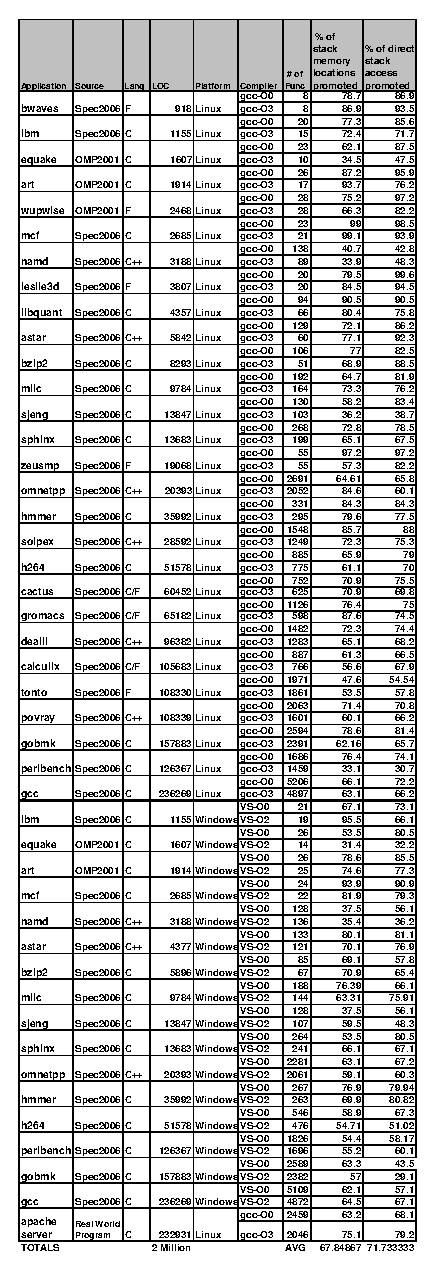
\includegraphics [width=0.7\linewidth] {figures/EPS/appTablenew2.eps} 
%\vspace{-3ex}
\caption { \textit{Benchmarks Table}}
\label{fig:appTable}
}
\vspace{-2ex}
\end{figure}


Algorithm~\ref{fig:algpartition} provides a formal description of the method for computing partitions for a memory location \emph{loc}. We begin with an empty partition. We analyze a store instruction, say \emph{ds}. If \emph{ds} is a direct addressing mode instruction then it is added to the DirectAcc set; otherwise it is added to BeginSet (Line 9-12). Load instructions using direct addressing where \emph{ds} is one of the reaching definitions are added to the DirectAcc set of the partition (Line 16-18). The remaining reaching definitions at these load instructions are added to the analysis list (Line 19-20). If \emph{ds} uses a direct addressing mode, indirect load and store instructions with \emph{ds} as one of the reaching definitions are added to the EndSet (Line 24-26). For indirect stores, the symbol need not be stored back to the memory (Line 22-23). As with the direct loads, the rest of the reaching definitions are added to the analysis list (Line 27-29). This analysis is applied repeatedly until the analysis list is empty. At that point, we have one independent partition. We repeatedly obtain new partitions until there are no more direct stores or indirect stores to analyze. 

We implement a simple benefit-cost model to determine whether the symbol promotion should be carried out for a particular partition. In a partition, the size of DirectAcc set is the number of memory accesses replaced by symbol accesses. We define $Freq_{i}$ as the statically determined execution frequency at program point i. Hence, the benefit of symbol promotion in terms of eliminated memory references:

{\begin{scriptsize}
\begin{equation} 
\begin{split}
Benefit= \sum_{i | i \in DirectAcc}\{ (Freq_{i})\} 
\end{split}
\end{equation} 
\end{scriptsize}}

One promoting load/store is needed for each element of BeginSet and Endset, consequently, the cost:

{\begin{scriptsize}
\begin{equation} 
\begin{split}
Cost= \sum_{i | i \in BeginSet}\{ (Freq_{i})\} + \sum_{i | i \in EndSet}\{ (Freq_{i})\} 
\end{split}
\end{equation} 
\end{scriptsize}}
We calculate the net benefit of each partition as \emph{Benefit - Cost}. Symbol promotion is carried out in a partition only if the net benefit is positive. 

